% !TeX root = ..\rapport_13_2.tex
\section{White box test\label{chap:white_box}}
\subsection{createInitials()}
For at garantere, at createInitials() fungerer som angivet i kommentaren over metodedefinitionen i klassen Employee (og dermed som forventet), skal vi sikre, at initialerne genereres i den rækkefølge, der er defineret af den kommentar, og at metoden kaster en undtagelse, når det forventes.
\begin{figure}[H]
    \centering
    \caption{Execution paths i createInitials()}
    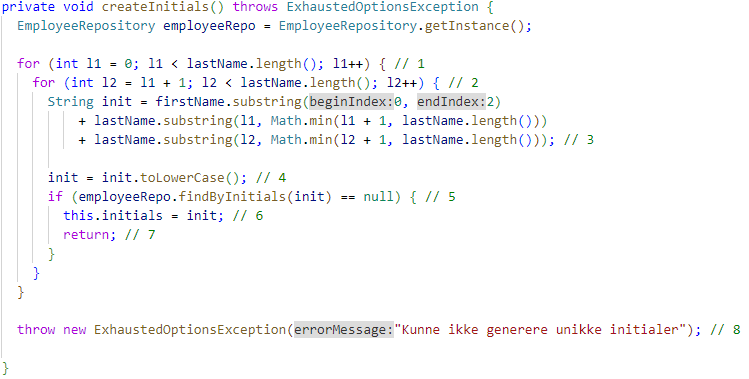
\includegraphics[width = \textwidth, keepaspectratio]{ImplementationAndTest/Diagrams/wb_create_initials.png}
    \label{fig:ep_create_initials}
\end{figure}
\noindent
For at gøre det bruger vi de execution paths, der er angivet i fig. \ref{fig:ep_create_initials} og skriver input-sæt, der sikrer, at alle execution paths dækkes.
\begin{table}[H]
\centering
\begin{tblr}{
  cells = {c},
  hline{1-2} = {-}{},
}
Execution path                                & Input set & Input property                                                                                 \\
1 (true), 2 (true), 3, 4, 5 (true), 6, 7         & A         & {There are fewer than 18 employees registered with\\first name "Michael", last name "Laudrup"} \\
1 (true), 2 (true), 3, 4, 5 (false), 8 & B         & {There are exactly 18 employees registered with first name\\~"Michael", last name "Laudrup"}   \\
1 (true), 2 (false), 8                 & C         & {There are exactly five employees registered with \\first name "Michael", last name "Laudrup"}   \\
1 (false), 8                              & B         & {There are exactly 18 employees registered with\\first name "Michael", last name "Laudrup"}    
\end{tblr}
\end{table}

\begin{table}[H]
\centering
\begin{tblr}{
  cells = {c},
  hline{1-2} = {-}{},
}
Input set & Input Data                                                                                  & Expected result                                                                                     \\
A         & {The employee repository is empty, \\and 18 employees named Michael Laudrup\\~are added.}   & {Initials are generated according to the description \\in the comment above createInitials.}        \\
B         & {The employee repository has 18 employees named\\~Michael Laudrup, and another is created.} & {An ExhaustedOptionsException is thrown with \\the message "Kunne ikke generere unikke initialer".}  \\
C         & {The employee repository has five employees named\\~Michael Laudrup, and another is created.} & {The sixth Michael Laudrup gets the initials miau} 
\end{tblr}
\end{table}
\subsection{generateProjectNumber()} 
\begin{figure}[H]
    \centering
    \caption{Execution paths i generateProjectNumber()}
    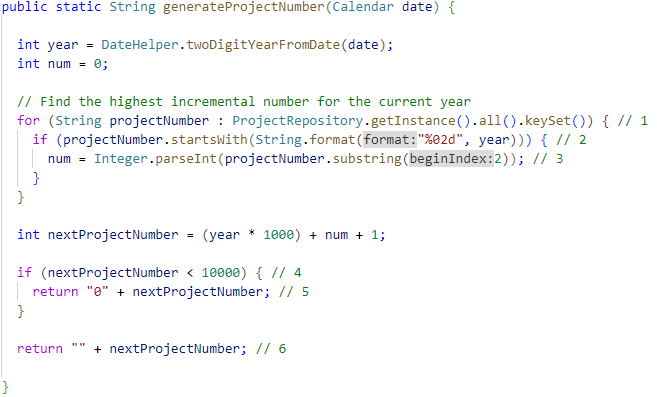
\includegraphics[width = \textwidth, keepaspectratio]{ImplementationAndTest/Diagrams/wb_genProjNum.png}
    \label{fig:ep_generate_project_number}
\end{figure}
\begin{table}[H]
\centering
\begin{tblr}{
  cells = {c},
  hline{1-2} = {-}{},
}
Execution path                                                     & Input set & Input property                                                                                                                  \\
{1 (not empty), 2 (true), 3, 4 (true), 5, 6} & A         & {There are projects from the current year, and the\\final two digits of the current year are \\less than 10}                    \\
{1 (not empty), 2 (true), 3, 4 (false), 6}   & B         & {There are projects from the current year, and the\\final two digits of the current year are\\greater than 10}                  \\
{1 (not empty), 2 (false), 4 (true), 5, 6}         & C         & {There is a project from a different year than the \\current, and the final two digits of the current\\year are less than 10}   \\
{1 (not empty), 2 (false), 4 (false), 6}           & D         & {There is a project from a different year than the\\current, and the final two digits of the current\\year are greater than 10} \\
1 (empty), 4 (true), 5, 6                                       & E         & {There are no projects and the final two digits of the\\~current year are less than 10}                                         \\
1 (empty), 4 (false), 6                                          & F         & {There are no projects and the final two digits of the\\current year are greater than 10}                                       
\end{tblr}
\end{table}                

\begin{table}[H]
\centering
\begin{tblr}{
  cells = {c},
  hline{1-2} = {-}{},
}
Input set & Input data                                                                                                      & Expected result                             \\
A         & {The current year is 2002 and there are two projects from the \\same year with project numbers 02001 and 02002} & {A new project with project number\\~02003} \\
B         & {The current year is 2023 and there are two projects from the \\same year with project numbers 23001 and 23002} & {A new project with project number\\~23003} \\
C         & {The current year is 2001 and there is a project from 2022 \\with project number 22001}                         & {A new project with project number\\~01001} \\
D         & {The current year is 2023 and there is a project from 2022\\with project number 22001}                          & {A new project with project number\\~23001} \\
E         & The current year is 2001 and there are no projects                                                              & {A new project with project number\\~01001} \\
F         & The current year is 2023 and there are no projects                                                              & {A new project with project number\\~23001} 
\end{tblr}
\end{table}

\subsection{createProjectActivity() \label{chap:white_box_create_project_activity}} 
Der kan oprettes projektaktiviteter for et projekt objekt. For at oprette en projektaktivitet, kræves at en medarbejder er logget ind og der skal bruges en titel, start- og slutuge. Derudover er det kun projektledere der kan oprette aktiviteter, hvis der er tildelt en projektleder til projektet. Herunder i \ref{lst:create_project_activity_source} er et udsnit af Project.java, inklusiv metoden der laves white box test for. White box testen udføres i praksis med JUnit, med filen CreateProjectActivityTest.java.


\begin{listing}[H]
    \centering
    \caption{createProjectActivity() source code}\label{lst:create_project_activity_source}
    \begin{minted}[breaklines]{java}
public class Project implements ConvertibleToViewModelInterface {

  private Employee projectLeader;
  private List<ProjectActivity> activities = new ArrayList<ProjectActivity>();

  public ProjectActivity createProjectActivity(String title, String startWeek, String endWeek, Employee loggedInUser)
      throws AlreadyExistsException, OperationNotAllowedException, InvalidPropertyException {
        
    if (hasProjectLeader()) { //1
      if (!projectLeader.isSameAs(loggedInUser)) { //2
        throw new OperationNotAllowedException("Kun projektlederen kan oprette en projekt aktivitet for dette projekt"); //3
      }
    }
    
    if (hasProjectActivity(title)) { //4
      throw new AlreadyExistsException("Projekt aktivitet findes allerede"); //5
    }
    
    ProjectActivity activity = new ProjectActivity(title, startWeek, endWeek); //6
    this.activities.add(activity); //7

    return activity;
  }
  
}

    \end{minted}
\end{listing}
% This centering command centers everything from here and down
%\centering
\begin{table}[H]

\caption{Execution paths in createProjectActivity()}\label{tbl:create_project_activity_paths}
\begin{tblr}{
  cells = {l},
  hline{1-2} = {-}{},
}
Execution path & 
Input set & 
Input property \\

{1 (false), 4 (false), 6, 7} & A & 
{
    \texttt{projectLeader} is null, \\ 
    \texttt{activities} does not contain an activity with title \texttt{title}
} \\

{1 (false), 4 (true), 5} & B & 
{
    \texttt{projectLeader} is null, \\ 
    \texttt{activities} contains an activity with title \texttt{title}
} \\

{1 (true), 2 (false), 4 (false), 6, 7} & C & 
{
    \texttt{projectLeader} is the same object as \texttt{loggedInUser},\\ 
    \texttt{activities} does not contain an activity with title \texttt{title}
} \\

{1 (true), 2(false), 4 (true), 5} & D & 
{
    \texttt{projectLeader} is the same object as \texttt{loggedInUser}, \\ 
    \texttt{activities} contains an activity with title \texttt{title}
} \\

{1 (true), 2(true), 3} & E & 
{
    \texttt{projectLeader} is another employee object than \texttt{loggedInUser}, \\
    \texttt{activities} does not contain an activity with title \texttt{title}
}\\

\end{tblr}
\end{table}                

\begin{table}[H]
\centering
\caption{Input sets for createProjectActivity()}\label{tbl:create_project_activity_inputs}
\begin{tblr}{
  cells = {l},
  hline{1-2} = {-}{},
}
Input set & 
Input data & 
Expected result \\

A & 
{
    \texttt{projectLeader} is null \\
    \texttt{activities} is empty \\
    \texttt{title} = "Planlægning" \\
    \texttt{startWeek} = "2101" \\ 
    \texttt{endWeek} = "2103" \\
    \texttt{loggedInUser} = \{"mila"\}
} & 
{
    \texttt{activities} contains a project activity \\ 
    with \texttt{title} "Planlægning"
} \\

B & 
{
    \texttt{projectLeader} is null \\
    \texttt{activities} = ["Planlægning"] \\
    \texttt{title} = "Planlægning" \\
    \texttt{startWeek} = "2101" \\ 
    \texttt{endWeek} = "2103" \\
    \texttt{loggedInUser} = \{"mila"\}
} & 
{
    Exception with message \\ 
    "Projekt aktivitet findes allerede" is thrown
} \\

C & 
{
    \texttt{projectLeader} = \{"mila"\} \\
    \texttt{activities} is empty \\
    \texttt{title} = "Planlægning" \\
    \texttt{startWeek} = "2101" \\ 
    \texttt{endWeek} = "2103" \\
    \texttt{loggedInUser} = \{"mila"\}
} & 
{
    \texttt{activities} contains a project activity \\ 
    with \texttt{title} "Planlægning"
} \\

D & 
{
    \texttt{projectLeader} = \{"mila"\} \\
    \texttt{activities} = ["Planlægning"] \\
    \texttt{title} = "Planlægning" \\
    \texttt{startWeek} = "2101" \\ 
    \texttt{endWeek} = "2103" \\
    \texttt{loggedInUser} = \{"mila"\}
} & 
{
    Exception with message \\ 
    "Projekt aktivitet findes allerede" is thrown
} \\

E & 
{
    \texttt{projectLeader} = \{"brla"\} \\
    \texttt{activities} is empty \\
    \texttt{title} = "Planlægning" \\
    \texttt{startWeek} = "2101" \\ 
    \texttt{endWeek} = "2103" \\
    \texttt{loggedInUser} = \{"mila"\}
} & 
{
    Exception with message \\ 
    "Kun projektlederen kan oprette en projekt aktivitet for dette projekt" is thrown
} \\

\end{tblr}
\end{table}

\subsection{findWorkTimeRegistrationById()}

For et givet projekt kan der oprettes projektaktiviteter, hvor en medarbejder kan angive mængden af arbejdstid han/hun har brugt på den pågældende aktivitet. Disse registreringer af arbejdstid bliver gemt med et id-nummer, som består af de positive naturlige tal og løber fra 1 og op. Dermed er det muligt at finde specifikke registreringer ud fra id-nummeret, og hertil benyttes metoden \texttt{findWorkTimeRegistrationById()}. 

Såfremt at id nummeret man søger efter, matcher det af en arbejdstidsregistrering, returneres den pågældende registrering. Hvis ikke der er et match, kastes en NotFoundException. Dette tester vi

